\documentclass[border=10pt]{standalone}

\usepackage{tikz}
\usepackage{tikzsymbols}
\usetikzlibrary{calc,patterns,shapes.geometric}

\def\centerarc[#1](#2)(#3:#4:#5){\draw[#1] ($(#2)+({#5*cos(#3)},{#5*sin(#3)})$) arc (#3:#4:#5);}

\begin{document}
	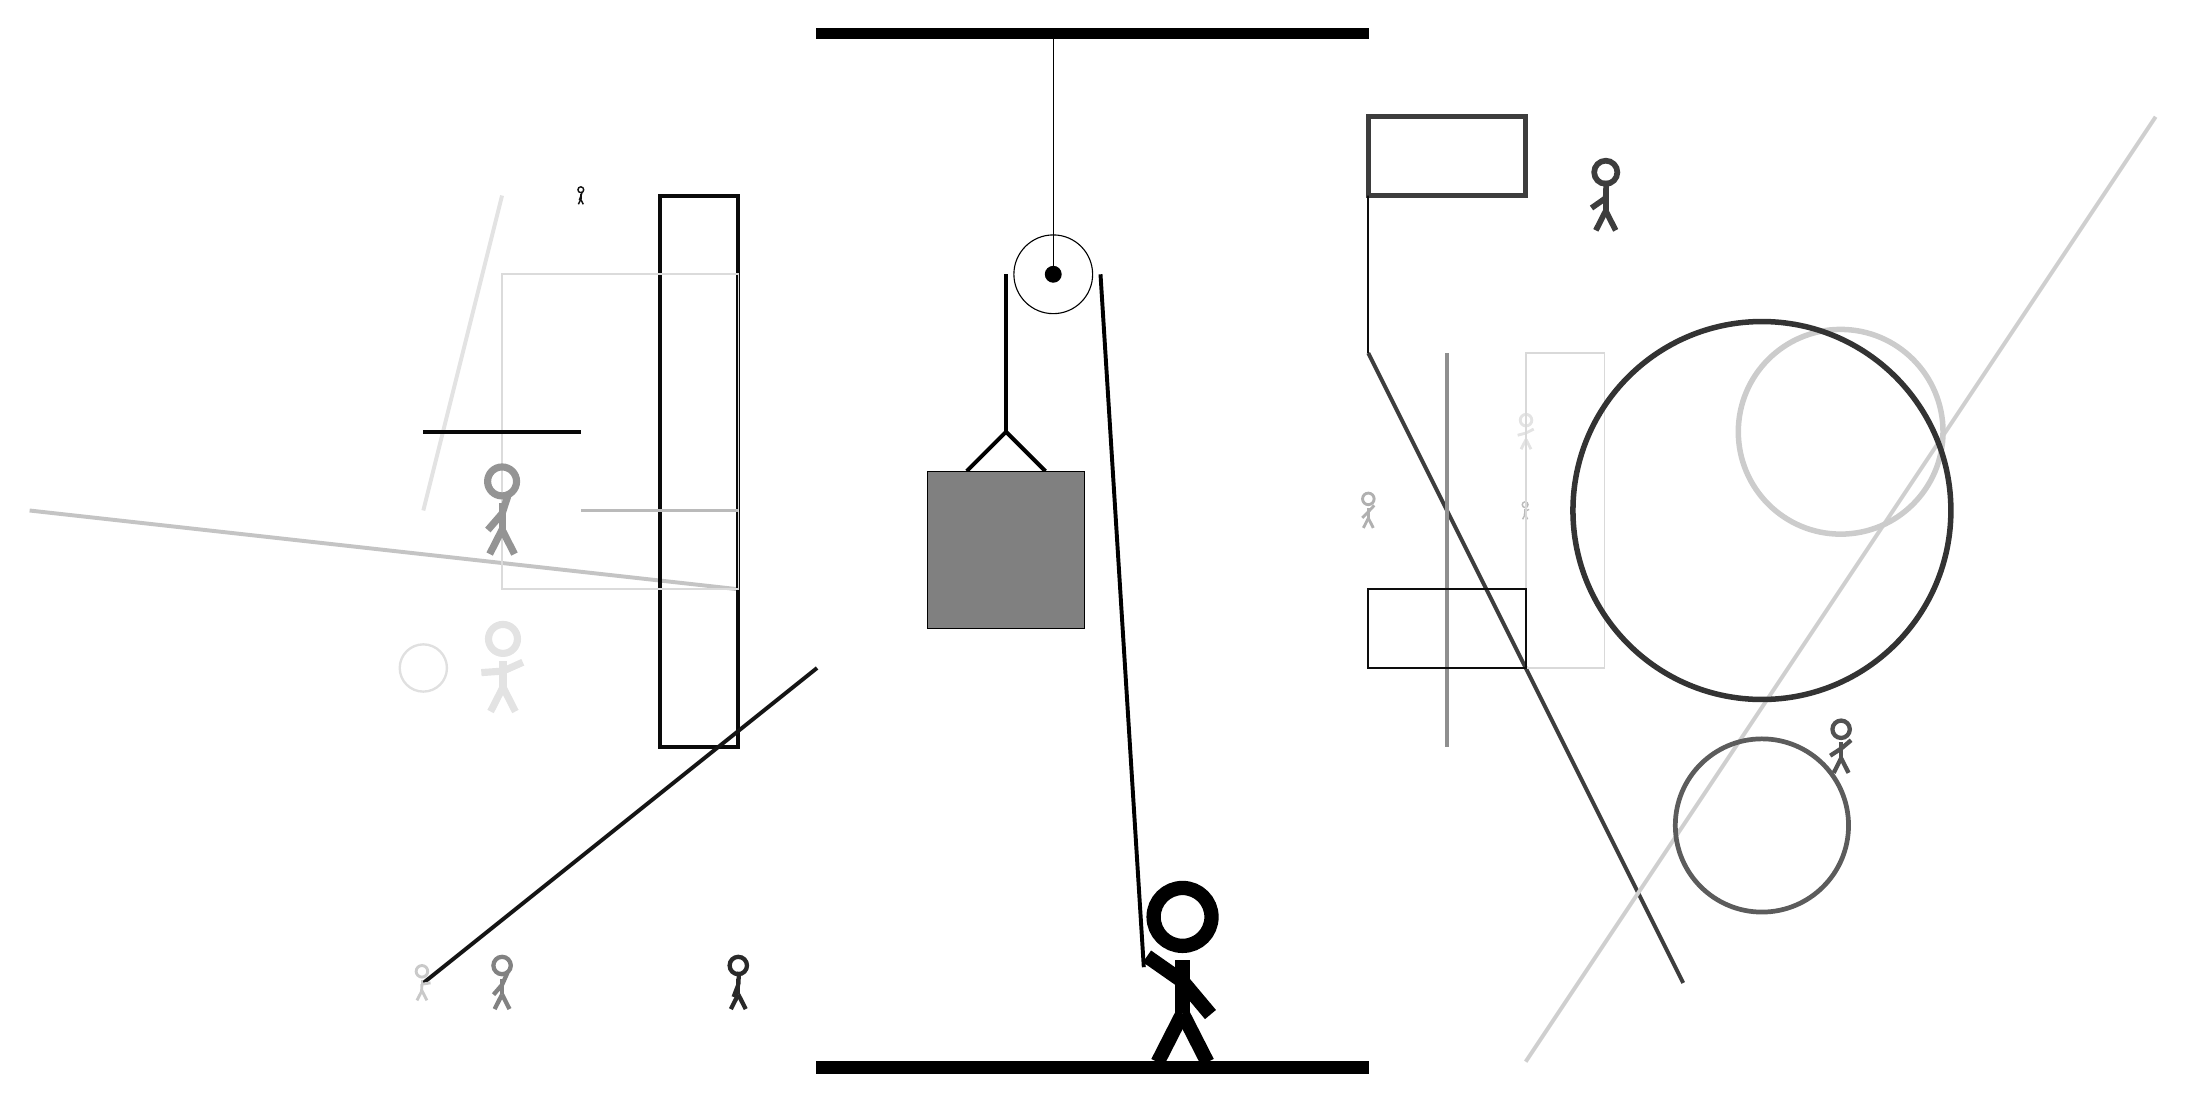
\begin{tikzpicture}
		%%%%% START %%%%%
		
		\draw[fill=black] (-2, 10) rectangle (5, 10.125);
		
		\draw (1, 7) circle (0.5);
		\draw[fill=black] (1, 7) circle (0.1);
		\draw (1, 10) -- (1, 7);
		
		\draw[line width=0.5mm, color=black!76](5, 6) -- (9, -2);
		
		\node[line width=0.5mm, color=black!11] at (7, 5) {\Strichmaxerl[2][15][27]};
		\draw[line width=0.5mm, color=black!44](6, 6) -- (6, 1);
		\draw[line width=0.5mm, color=black!23](-3, 3) -- (-12, 4);
		\node[line width=0.7mm, color=black!68] at (11, 1) {\Strichmaxerl[3][33][40]};
		\draw[line width=0.5mm, color=black!19](7, -3) -- (15, 9);
		\node[line width=0.5mm, color=black!49] at (-6, -2) {\Strichmaxerl[3][49][66]};
		\draw[line width=0.5mm, color=black!11](-7, 4) -- (-6, 8);
		\node[line width=0.7mm, color=black!11] at (-6, 2) {\Strichmaxerl[5][4][24]};
		\node[line width=0.2mm, color=black!76] at (8, 8) {\Strichmaxerl[4][35][88]};
		\draw[line width=0.5mm, color=black!96] (-3, 1) rectangle (-4, 8);
		\node[line width=0.4mm, color=black!27] at (7, 4) {\Strichmaxerl[1][78][23]};
		\draw[line width=0.2mm, color=black!15] (7, 6) rectangle (8, 2);
		
		\draw [line width=0.7mm, color=black!20](11, 5) circle (1.3);
		\draw [line width=0.3mm, color=black!12](-7, 2) circle (0.3);
		\draw[line width=0.2mm, color=black!14] (-3, 7) rectangle (-6, 3);
		\draw[line width=0.3mm, color=black!95] (5, 3) rectangle (7, 2);
		
		\draw[line width=0.6mm, color=black!76] (5, 9) rectangle (7, 8);
		\draw[line width=0.5mm, color=black!92](-7, -2) -- (-2, 2);
		\draw [line width=0.7mm, color=black!80](10, 4) circle (2.4);
		\node[line width=0.7mm, color=black!42] at (-6, 4) {\Strichmaxerl[5][49][72]};
		
		\draw[line width=0.5mm, color=black!27](-5, 4) -- (-3, 4);
		
		\node[line width=0.3mm, color=black!31] at (5, 4) {\Strichmaxerl[2][45][47]};
		\draw [line width=0.6mm, color=black!64](10, 0) circle (1.1);
		\node[line width=0.2mm, color=black!21] at (-7, -2) {\Strichmaxerl[2][87][9]};
		\node[line width=0.2mm, color=black!93] at (-5, 8) {\Strichmaxerl[1][69][72]};
		\node[line width=0.7mm, color=black!84] at (-3, -2) {\Strichmaxerl[3][69][87]};
		\draw[line width=0.5mm, color=black!97](-7, 5) -- (-5, 5);
		\draw[line width=0.3mm, color=black!95] (5, 8) rectangle (5, 6);
		
		\draw[line width=0.5mm] (-0.1, 4.5) -- (0.4, 5.0) -- (0.9, 4.5);
		\draw[fill=black!50] (-0.6, 4.5) rectangle (1.4, 2.5);
		
		\draw[line width=0.5mm] (0.4, 7) -- (0.4, 5.0);
		\centerarc[line width=0.5mm](1, 7)(0:180:0.6);
		\draw[line width=0.5mm](1.6, 7) -- (2.15, -1.8);
		
		\node at (2.6, -1.9) {\Strichmaxerl[10][-35][-50]};
		
		\draw[fill=black] (-2, -3) rectangle (5, -3.15);
		
		%%%%% END %%%%%
	\end{tikzpicture}
\end{document}